\documentclass{beamer}
\setbeameroption{show notes} % un-comment to see the notes
\setbeamertemplate{itemize items}[triangle]

\mode<presentation>{ 
  %\usetheme{AnnArbor}
  %\usetheme{Antibes}
  %\usetheme{Bergen}
  %\usetheme{Berkeley}
  %\usetheme{Berlin}
  %\usetheme{Boadilla}
  %\usetheme{boxes}
  %\usetheme{CambridgeUS}
  %\usetheme{Copenhagen}
  %\usetheme{Darmstadt}
  %\usetheme{default}
  %\usetheme{Frankfurt}
  %\usetheme{Goettingen}
  %\usetheme{Hannover}
  %\usetheme{Ilmenau}
  %\usetheme{JuanLesPins}
  %\usetheme{Luebeck}
  \usetheme{Madrid}
  %\usetheme{Malmoe}
  %\usetheme{Marburg}
  %\usetheme{Montpellier}
  %\usetheme{PaloAlto}
  %\usetheme{Pittsburgh}
  %\usetheme{Rochester}
  %\usetheme{Singapore}
  %\usetheme{Szeged}
  %\usetheme{Warsaw}
    
  \usecolortheme{default}
  %\usecolortheme{albatross}
  %\usecolortheme{beaver}
  %\usecolortheme{beetle}
  %\usecolortheme{crane}
  %\usecolortheme{dolphin}
  %\usecolortheme{dove}
  %\usecolortheme{fly}
  %\usecolortheme{lily}
  %\usecolortheme{orchid}
  %\usecolortheme{rose}
  %\usecolortheme{seagull}
  %\usecolortheme{seahorse}
  %\usecolortheme{whale}
  %\usecolortheme{wolverine}
  
  \usefonttheme{default}  % or try serif, structurebold, ...
  \setbeamertemplate{navigation symbols}{}
}

%\usepackage[spanish, es-tabla]{babel} % provide language hyphenation
\usepackage[utf8]{inputenc} % use UTF8 encoding

\usepackage{fancyhdr} % allows fancy headers
\usepackage{xcolor} % define colors

\usepackage{amsmath} % mathematical equations
\usepackage{amssymb} % add maths symbols
\usepackage{mathtools} % more maths symbols

\usepackage{graphicx} % add figures
\usepackage{caption} % caption customization
\usepackage{subcaption} % subfigures caption customization
\usepackage{geometry} % page layout modification
\usepackage{tikz} % tikz figures

%\usepackage{enumitem} % enumerate customization
\usepackage{glossaries} % add glossaries
\usepackage{listings} % code listing
%\usepackage{algorithm}
%\usepackage{algpseudocode}
\usepackage[ruled, linesnumbered]{algorithm2e}

\usepackage{cite} % citing
\usepackage{hyperref} % produces hypertext links
\usepackage{verbatim} % multiline comments

\usepackage{multirow} % more table options (e.g. multitables)
\usepackage{booktabs} % even more table options

\usepackage{todonotes} % todo notes

\newcommand{\Nn}{\mathcal{N}}
\newcommand{\Cc}{\mathcal{C}}
\newcommand{\Ee}{\mathcal{E}}
\newcommand{\bs}{\boldsymbol}
\newcommand{\defi}{\vcentcolon=}
\renewcommand{\it}{\textit}

\usepackage{lmodern}
\usepackage{picture}
%\usepackage{pgfpages}
%\setbeameroption{show notes on second screen=right}

\setbeamertemplate{enumerate items}[default]
\renewcommand\mathfamilydefault{\rmdefault}

\title[GraphSLAM Implementation]{Thesis Defense}
\subtitle{GraphSLAM Algorithm Implementation for Solving\\Simultaneous Localization and Mapping}
\author[Franco Curotto]{}
\institute[UCHILE - FCFM - DIE]{Departamento de Ingeniería Eléctrica\\Facultad de Ciencias Físicas y Matemáticas\\Universidad de Chile}
\date{\vspace{0em}April 18, 2016}

\begin{document}
	
\begin{frame}
\author{
\vspace{-1em}
\hspace{-4em}
\begin{tabular}{rl} 
 \textbf{Author:}  & Franco Curotto \\
 \textbf{Thesis Adviser:} & Martin Adams \\ 
 \textbf{Commission Members:} & Marcos Orchard \\
 & Jorge Silva
\end{tabular}
\vspace{0em}
}
    
\includegraphics[width=0.4\textwidth]{img/fcfm_die.pdf}
    \titlepage
\end{frame}

% \note[itemize]{
% \item You may be wondering what GraphSLAM and SLAM
% \item My work is ... in the field of robotics
% }

% \begin{frame}{Motivation}
% \begin{columns}[T]
% \column{0.5\textwidth}
% \centering
% \textbf{Robots Before}\\
% \vspace{1em}
% 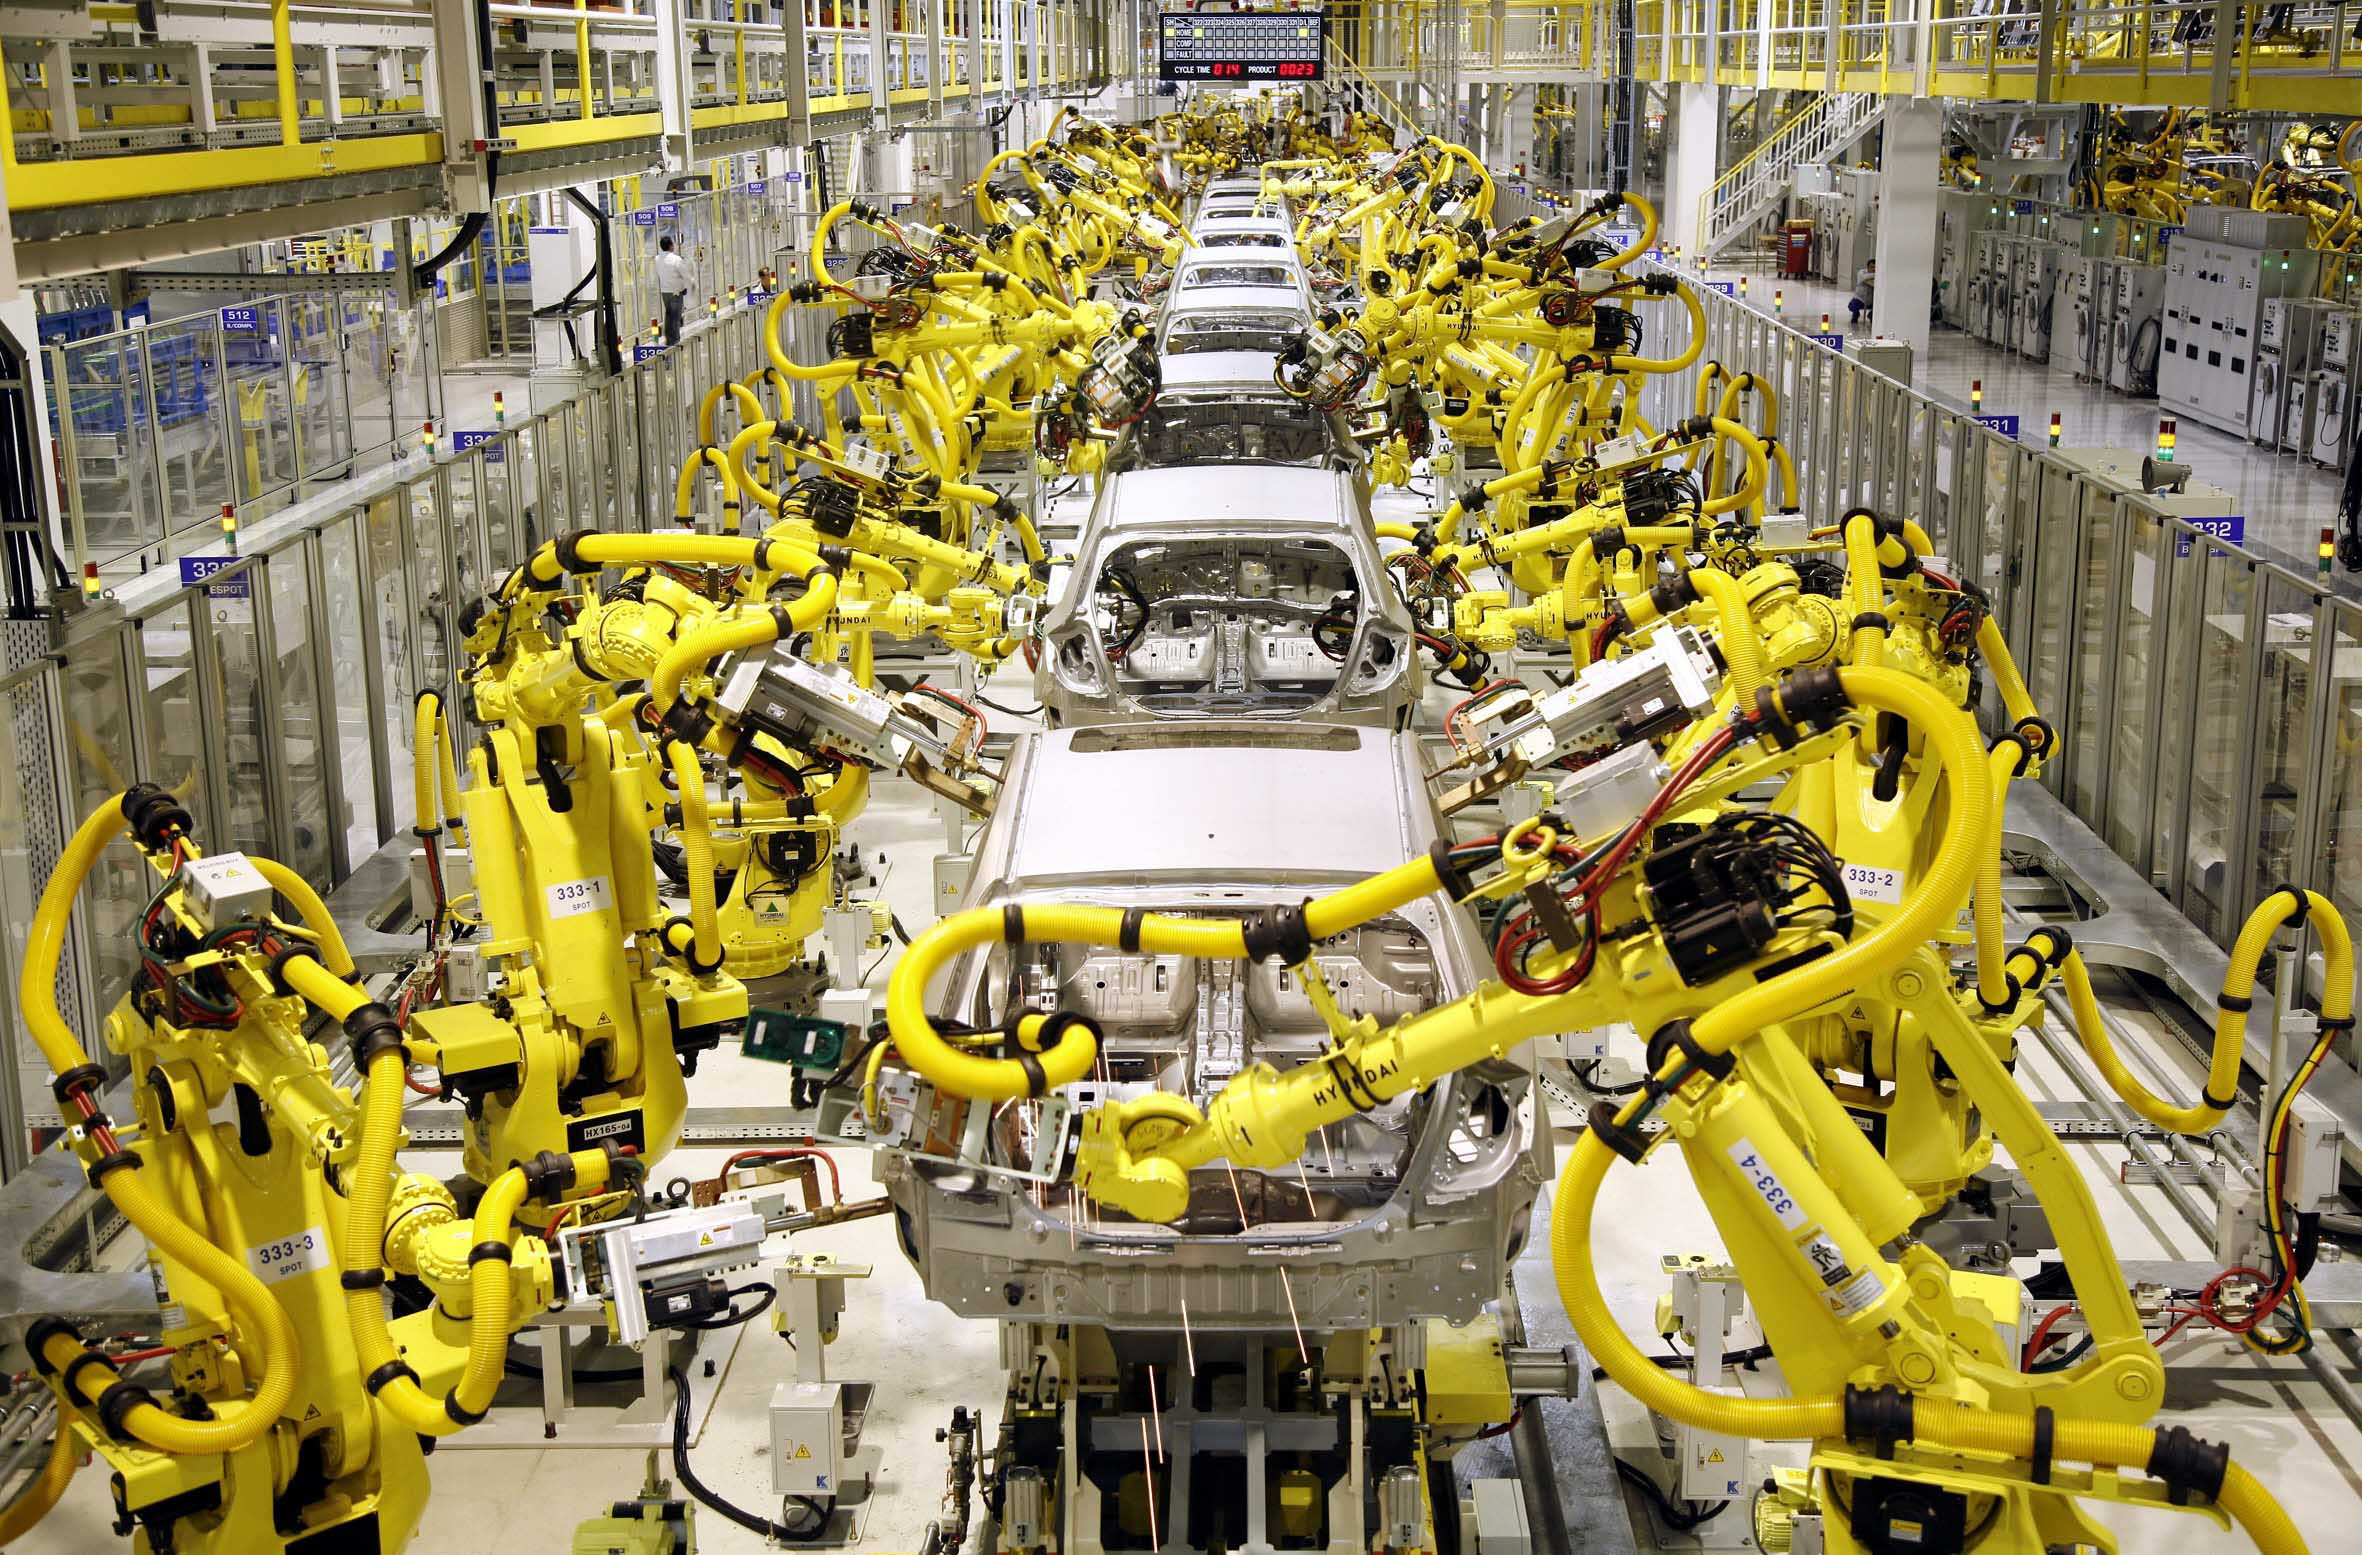
\includegraphics[height=0.37\textheight]{img/assembly.jpg}\\
% \vspace{1em}
% 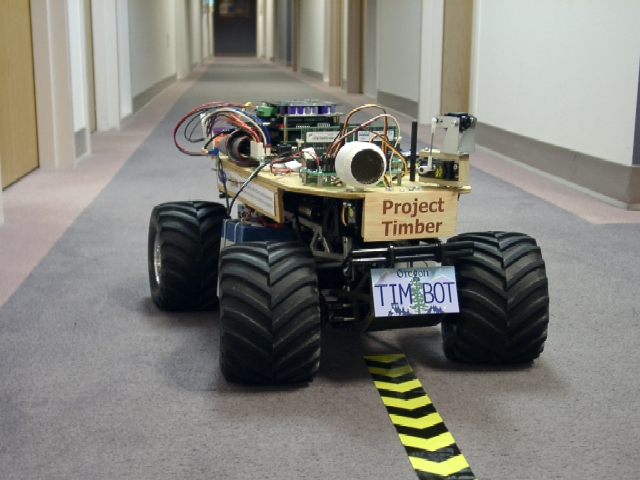
\includegraphics[height=0.37\textheight]{img/timbot.jpg}
% \pause
% \column{0.5\textwidth}
% \centering
% \vspace{-2pt}
% \textbf{Robots Today}\\
% \vspace{1em}
% 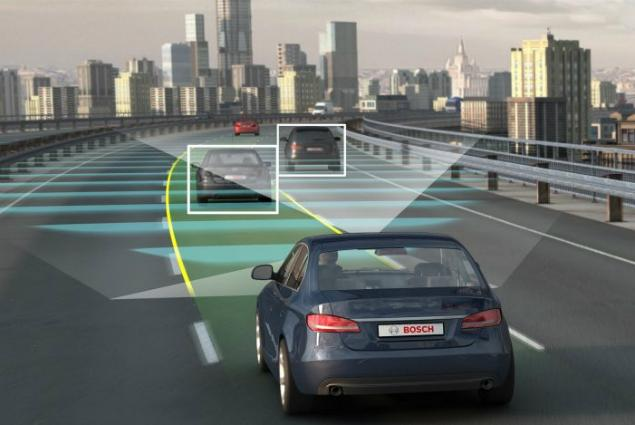
\includegraphics[height=0.37\textheight]{img/selfdriving.jpg}\\
% \vspace{1em}
% 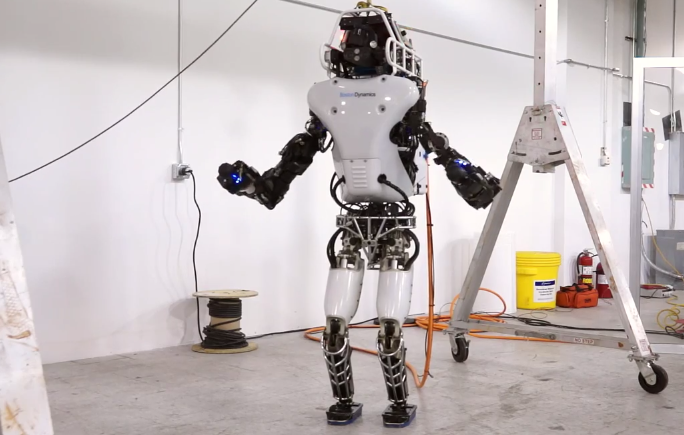
\includegraphics[height=0.37\textheight]{img/atlas2.png}
% \end{columns}
% \end{frame}

% \note[itemize]{
% \item Robots in the past were restricted to do simple, repetitive tasks, and were either stationary [reference photo], or had limited mobility, usually by following a reference [reference photo]. 
% \item Robots nowadays need to be much more versatile, autonomous and robust [reference photos].
% \item In particular robots must be able to move freely in an open environment.
% }

\begin{frame}{Motivation}
\begin{center}
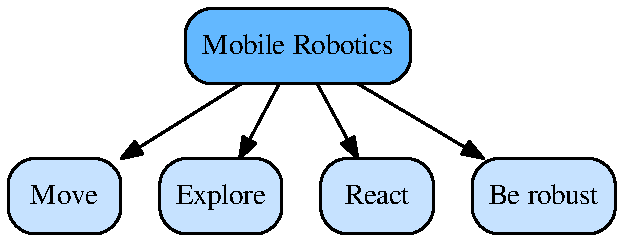
\includegraphics[width=0.7\textwidth]{dot/mobile.pdf}\\
\end{center}
\begin{columns}
\column{0.5\textwidth}
\centering
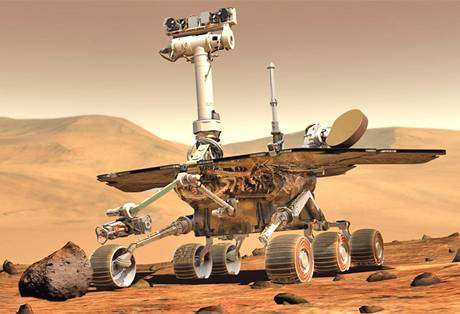
\includegraphics[width=0.8\textwidth]{img/mars-rover.jpg}\\
\column{0.5\textwidth}
\centering
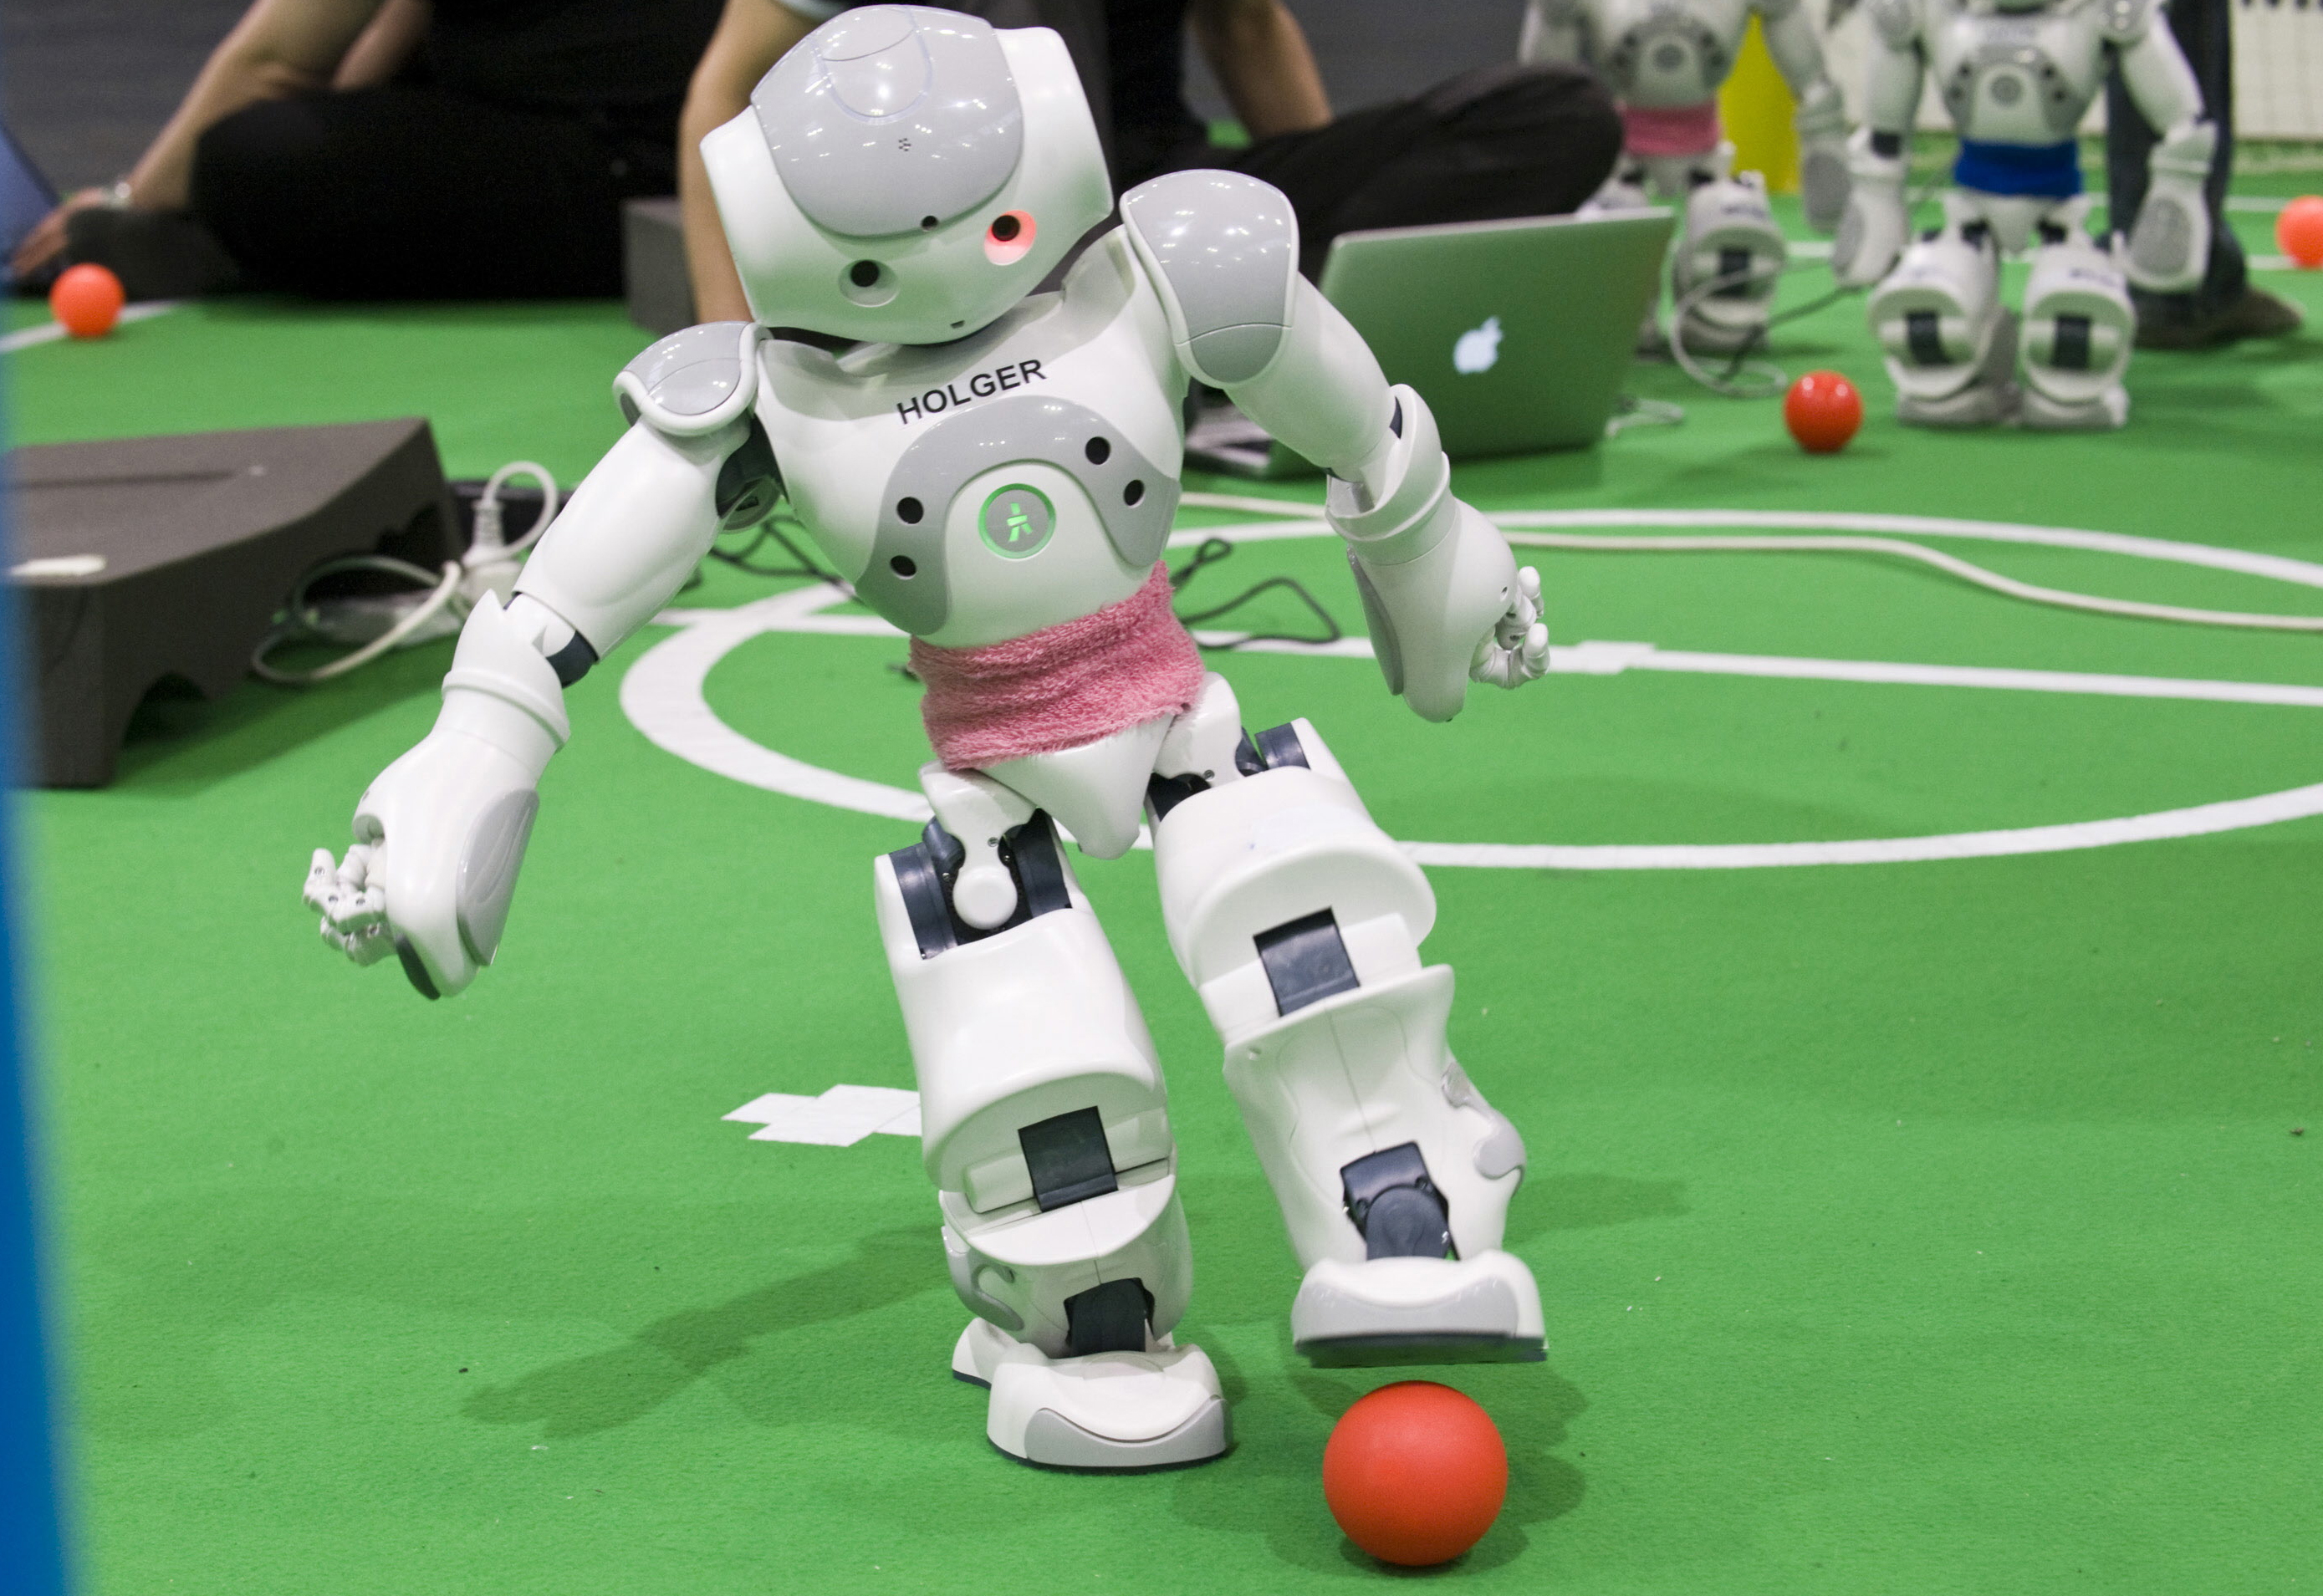
\includegraphics[width=0.8\textwidth]{img/football.jpg}\\
\end{columns}
%\vspace{1em}
% \begin{block}{Mobile Robots}
% \begin{itemize}
% \item \textbf{Move} around known environments without getting lost.
% \item \textbf{Explore} new environments, and ``remember'' them. 
% \item \textbf{React} to unexpected changes.
% \item  Perform their tasks in \textbf{suboptimal conditions}. 
% \end{itemize}
% \end{block}
\end{frame}

% \note[itemize]{
% \item A robot must be able to identify where in the scenario he is standing on.
% \item For example if you buy a robot for your house, he never has seen your house before, so he must be able to explore it and remember it for later use.
% \item For example when the environment changes, or when there is something moving on the room.
% }

\begin{frame}{Simultaneous Localization and Mapping}
\begin{block}{SLAM}
\begin{center}
\textit{
The problem were an agent must simultaneously estimate its current position (localization), and construct a map of its environment (mapping)}
\end{center}
\end{block}
\vspace{1em}
\pause
\begin{columns}
\column{0.5\textwidth}
We have (information):
\begin{itemize}
\item Robot odometry
\item Landmarks measurements
\end{itemize}
\vspace{1em}
\centering
%
\includegraphics[height=7em]{img/encoder.png}
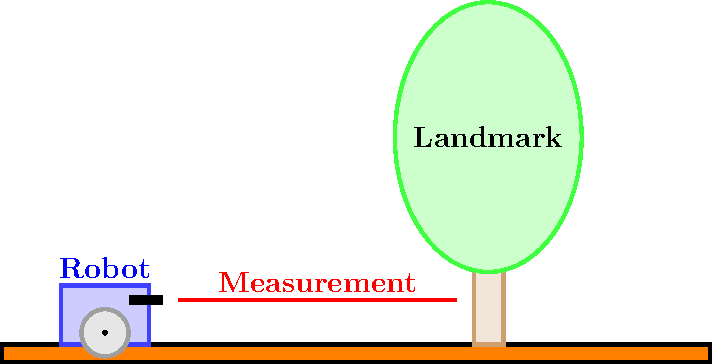
\includegraphics[width=\textwidth]{tikz/landmark.pdf}\\
\column{0.5\textwidth}
We need (states):
\begin{itemize}
\item Robot position
\item Robot orientation
\makebox(0,0){\put(0,2.2\normalbaselineskip){%
               $\left.\rule{0pt}{1.1\normalbaselineskip}\right\}$ Robot pose}}
\item Landmarks position
\end{itemize}
\vspace{42pt}
\centering
%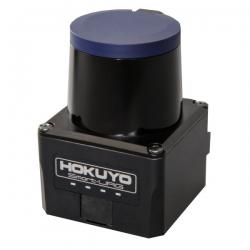
\includegraphics[height=8em]{img/Hokuyo-UST-20LX.jpg}
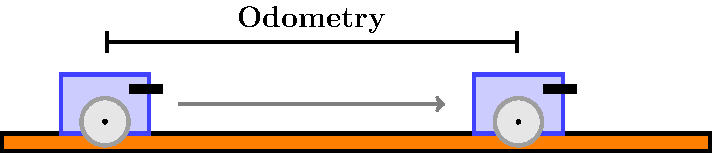
\includegraphics[width=\textwidth]{tikz/odometry.pdf}\\
\end{columns}
% \begin{block}{Odometry and Measurements}
% Sensors can be used to:
% \begin{itemize}
% \item Keep track of the robot movements (odometry)
% \item Sense nearby objects positions (measurements)
% \end{itemize}
% Sensors are noisy. We can use probabilistic methods to improve sensors estimates.
% \end{block}
% \begin{columns}
% \column{0.5\textwidth}
% 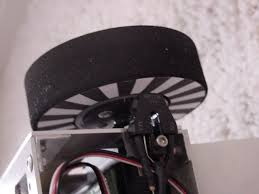
\includegraphics[width=0.6\textwidth]{img/encoders.jpg}
% \centering
% \column{0.5\textwidth}
% \centering
% 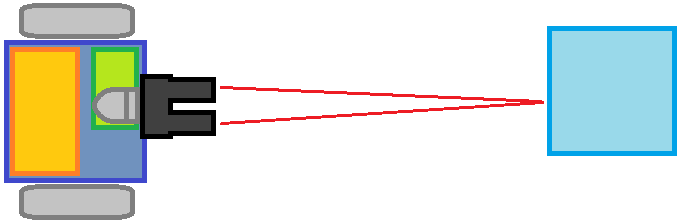
\includegraphics[width=0.8\textwidth]{img/laser.png}
% \end{columns}
\end{frame}

\begin{frame}{Simultaneous Localization and Mapping}
% \begin{columns}
% \column{0.5\textwidth}
% Motion Model
% \begin{equation}
% \end{equation}
% \column{0.5\textwidth
% Measurement Model
% \end{columns}
% Both contaminated by (Gaussian) noise.
Motion Model:
\begin{equation*}
\bs{x}_k = \bs{g}(\bs{u}_k, \bs{x}_{k-1}) + \bs{\delta}_k
\label{eq:motion-model}
\end{equation*}  
\centering
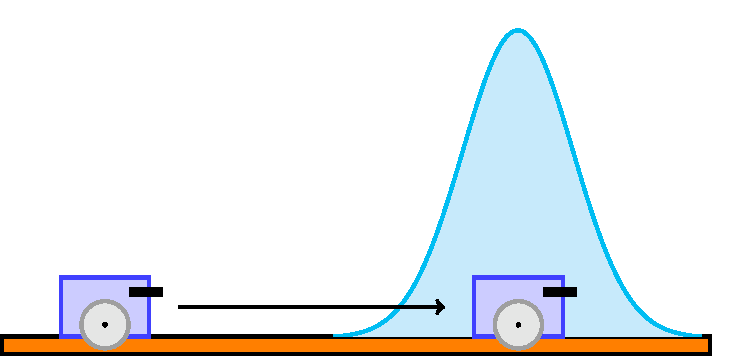
\includegraphics[width=0.47\textwidth]{tikz/motion.pdf}\\
%\pause
\raggedright
Measurement Model:
\begin{equation*}
\bs{z}_k^i = \bs{h}(\bs{x}_k,\bs{m}_j,i) + \bs{\varepsilon}_k^i
\label{eq:measurement-model}
\end{equation*}
\vspace{-1em}
\begin{columns}
\column{0.7\textwidth}
\raggedleft
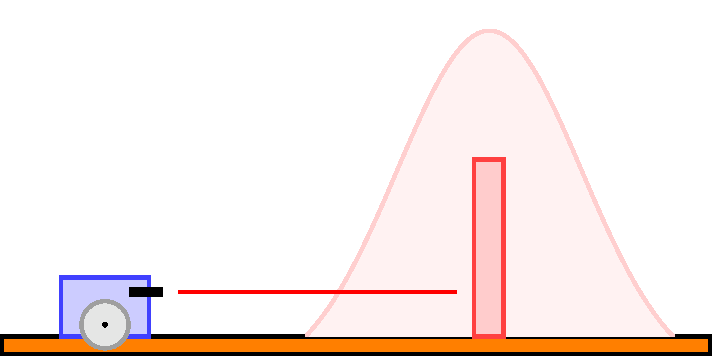
\includegraphics[width=0.67\textwidth]{tikz/measurements.pdf}
\column{0.3\textwidth}
%\begin{block}{}
Both contaminated with Gaussian noise.
%\end{block}
\end{columns}
\end{frame}

\begin{frame}{GraphSLAM}
%\begin{block}{}
GraphSLAM: SLAM $\Rightarrow$ graph
%\begin{itemize}
%\item Nodes represents robot \textbf{poses} or \textbf{landmarks}.
%\item Edges represents \textbf{robot} odometry or \textbf{measurements}.
%\end{itemize}
%\end{block}
\begin{center}
\includegraphics<1>[width=0.6\textwidth]{tikz/graphslam01.pdf}
\includegraphics<2>[width=0.6\textwidth]{tikz/graphslam02.pdf}
\includegraphics<3>[width=0.6\textwidth]{tikz/graphslam03.pdf}
\includegraphics<4>[width=0.6\textwidth]{tikz/graphslam04.pdf}
\includegraphics<5>[width=0.6\textwidth]{tikz/graphslam05.pdf}
\includegraphics<6>[width=0.6\textwidth]{tikz/graphslam06.pdf}
\includegraphics<7>[width=0.6\textwidth]{tikz/graphslam07.pdf}
\includegraphics<8>[width=0.6\textwidth]{tikz/graphslam08.pdf}
\includegraphics<9->[width=0.6\textwidth]{tikz/graphslam09.pdf}
\end{center}
\pause[10]
\begin{columns}
\column{0.5\textwidth}
Nodes are: Robot poses, or
\hphantom{Nodes are:} Landmarks positions
\column{0.5\textwidth}
Edges are: Odometry, or \hphantom{W}
\hphantom{Edges are:} Measurements
\end{columns}
\vspace{1em}
\begin{block}{}
Goal: Find the graph that more accurately represents the data.
\end{block}
\end{frame}

\begin{frame}{Mathematical Formulation of GraphSLAM}
%\begin{block}{}
%We want to find the maximum likelihood of posterior probability:
%\begin{equation*}
%p(\bs{x}_{0:k},\bs{m}|\bs{z}_{1:k},\bs{u}_{1:k})
%\end{equation*} 

%Which can be formulated as:
%\begin{equation*}
%F(\bs{y}) \defi -\log(p(\bs{y}|\bs{z}_{1:k},\bs{u}_{1:k})) = \sum_{\left<i,j\right>\in\Ee}\bs{e}_{ij}(\bs{y})^T\bs{\Omega}_{ij} \bs{e}_{ij}(\bs{y}) 
%\end{equation*}
%\pause
%\end{block}

SLAM posterior probability:
\begin{center}
\includegraphics<1>[width=0.5\textwidth]{tikz/likelihood1.pdf}
\includegraphics<2->[width=0.5\textwidth]{tikz/likelihood2.pdf}
\end{center}
\onslide<3->{
Using models in $-\log(p(\bs{y}|\bs{z}_{1:k},\bs{u}_{1:k}))$:
\begin{center}
\includegraphics<1-3>[width=0.5\textwidth]{tikz/log-likelihood1.pdf}
\includegraphics<4->[width=0.5\textwidth]{tikz/log-likelihood2.pdf}
\end{center}
We need the minimum of this expression.}

% \begin{block}{}
% \begin{itemize}
% \item $\bs{y}$: state vector (junction of robot poses and landmarks positions)
% \item $\bs{z_{1:k}}$: landmarks measurements
% \item $\bs{u_{1:k}}$: odometry measurements
% \item $\bs{e_{ij}}$: error function (difference between current estimate and data)
% \item $\bs{\Omega_{ij}}$: Information matrix of measurements
% \end{itemize}
% \end{block}
\end{frame}

% \begin{frame}{Mathematical Formulation of GraphSLAM}
% \begin{block}{Gauss-Newton algorithm}
% \begin{itemize}
% \item 1$^\circ$ order Taylor expansion around current estimate:
% \begin{equation}
% F(\breve{\bs{y}}+\bs{\Delta y}) = k + 2\bs{b} \bs{\Delta y} + \bs{\Delta y}^T \bs{H} \bs{\Delta y}
% \label{eq:taylor}
% \end{equation}
% \item Minimization of~\label{eq:taylor}:
% \begin{equation}
% \bs{H \Delta y}^* = -\bs{b}
% \label{eq:linear-system}
% \end{equation}
% \item Estimate update:
% \begin{equation}
% \bs{y}^* = \breve{\bs{y}}+ \bs{\Delta y}^*
% \label{eq:update}
% \end{equation}
% \end{itemize}
% \end{block}
% 
% \begin{block}{}
% \begin{itemize}
% \item $\breve{\bs{y}}$: current estimate
% \item $\bs{\Delta y}$: small disturbance around $\breve{\bs{y}}$
% \item $\bs{b}$: Information vector
% \item $\bs{H}$: Information matrix
% \item $\bs{y}^*$: New estimate
% \end{itemize}
% \end{block}
% \end{frame}

\begin{frame}{Mathematical Formulation of GraphSLAM}
\begin{itemize}
\onslide<1->{
\item g$^2$o: General Graph Optimization framework}
\vspace{1em}
\onslide<2->{
\item Gauss-Newton Algorithm:}
\begin{enumerate}
\onslide<2->{
\item Taylor Approximation:
\begin{equation*}
F(\breve{\bs{y}}+\bs{\Delta y}) = k + 2\bs{b} \bs{\Delta y} + \bs{\Delta y}^T \bs{H} \bs{\Delta y}
\end{equation*}}
\onslide<3->{
\item Minimization:
\begin{equation*}
\bs{H \Delta y}^* = -\bs{b}
\end{equation*}
\item Update:
\begin{equation*}
\bs{y}^* = \breve{\bs{y}}+ \bs{\Delta y}^*
\end{equation*}}
\end{enumerate}
\end{itemize}
\onslide<2->{
\begin{block}{}
\begin{itemize}
\item $\bs{b}$: Total system information vector
\item $\bs{H}$: Total system information matrix
\end{itemize}
\end{block}}
\end{frame}

\begin{frame}{Structure of the Linearized System}
Information matrix $\bs{H}$ is intrinsically \textit{\textbf{sparse}}.
\vspace{1em}

\centering
\includegraphics<1>[width=\textwidth]{tikz/matrix01.pdf}
\includegraphics<2>[width=\textwidth]{tikz/matrix02.pdf}
\includegraphics<3>[width=\textwidth]{tikz/matrix03.pdf}
\includegraphics<4>[width=\textwidth]{tikz/matrix04.pdf}
\includegraphics<5>[width=\textwidth]{tikz/matrix05.pdf}
\includegraphics<6>[width=\textwidth]{tikz/matrix06.pdf}
\includegraphics<7>[width=\textwidth]{tikz/matrix07.pdf}
\includegraphics<8>[width=\textwidth]{tikz/matrix08.pdf}
\includegraphics<9>[width=\textwidth]{tikz/matrix09.pdf}
\includegraphics<10>[width=\textwidth]{tikz/matrix10.pdf}
\end{frame}

% \begin{frame}{g$^2$o Protocol}
% \begin{center}
% \includegraphics<1>[width=0.7\textwidth]{tikz/protocol1.pdf}
% \includegraphics<2>[width=0.7\textwidth]{tikz/protocol2.pdf}
% \includegraphics<3>[width=0.7\textwidth]{tikz/protocol3.pdf}
% 
% \fontsize{8.5}{10.2}\selectfont
% %\scriptsize
% \begin{tabular}{|c|l|}
% \hline
% Graph Element & Notation\\
% \hline
% \onslide<1->{
% Pose Node & \texttt{VERTEX\_SE2 id x y a}\\
% Landmark Node & \texttt{VERTEX\_XY id x y}\\
% Fix a Node & \texttt{FIX id}\\}
% \onslide<2->{Odometry Edge} & \onslide<2->{\texttt{EDGE\_SE2 id1 id2 dx dy da ipxx ipxy ipxa ipyy ipya ipaa}}\\
% \onslide<3->{Measurement Edge} & \onslide<3->{\texttt{EDGE\_SE2\_XY id1 id2 dx dy ilxx ilxy ilyy}}\\
% \hline
% \end{tabular}
% \onslide<2->{
% \normalsize 
% \begin{block}{}
% One must specify the information matrix of edges.
% \end{block}}
% \end{center}
% \end{frame}
% 
\begin{frame}{Correspondence Problem}

\begin{columns}

\column{0.4\textwidth}
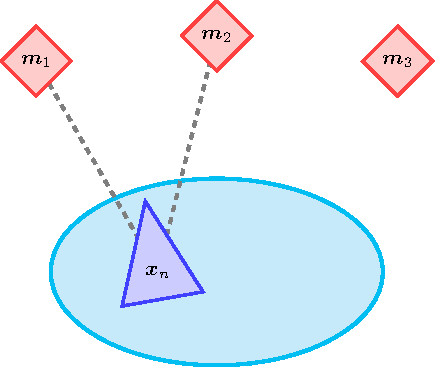
\includegraphics[width=\textwidth]{tikz/correspondence1.pdf}
\column{0.1\textwidth}
\centering
OR
\column{0.4\textwidth}
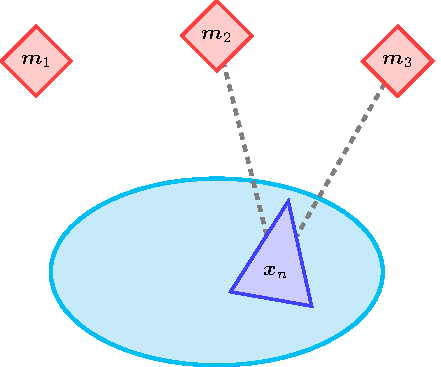
\includegraphics[width=\textwidth]{tikz/correspondence2.pdf}
\end{columns}

\vspace{2em}
\begin{itemize}
\setlength\itemsep{1em}
\item In the real world, \textbf{correspondence} between measurements and landmarks is \textbf{unknown}.
\item \textbf{Data association}: assignment of measurements to landmarks.
\end{itemize}
\end{frame}

\begin{frame}[fragile]{Correspondence Test}
\begin{block}{}
Premise: Compute the likelihood of two landmarks being the same.
\end{block}

\begin{equation*}
\pi_{i=j} \defi
\det(2\pi\bs{\Sigma}_{\bs{\Delta}_{i,j}})^{-\frac{1}{2}}
\exp\left\lbrace-\frac{1}{2}\bs{\mu}_{\bs{\Delta}_{i,j}}^T\bs{\Sigma}_{\bs{\Delta}_{i,j}}^{-1}\bs{\mu}_{\bs{\Delta}_{i,j}}\right\rbrace
\end{equation*}
\pause
We define threshold $\chi$.
\begin{columns}
\column{0.4\textwidth}
\begin{block}{}
If $\pi_{j=k} \geq \chi$:\\
\begin{itemize}
\item Merge landmarks $i$ and $j$
\end{itemize}
Else:\\
\begin{itemize}
\item Leave them separated
\end{itemize}
\end{block}
\end{columns}
\vspace{1em}
\pause
\begin{alertblock}{}
Problem: Matrix $\bs{\Sigma}_{\bs{\Delta}_{i,j}}$ is expensive to compute.
\end{alertblock}
\end{frame}

\begin{frame}{Distant Test}
\begin{block}{}
\begin{itemize}
\item Merges landmark according to the distance.
\item Avoids the computation of $\bs{\Sigma}_{\bs{\Delta}_{i,j}}$ for \textit{easy} cases.
\end{itemize}
\end{block}
\pause
Maximum distance at which associations can still be made:
\begin{equation*}
\bs{\mu}_{\bs{\delta}_{i,j}} = \sqrt{-2\sigma_{\bs{\delta}_{i,j}}^2\log(\sqrt{2\pi\sigma_{\bs{\delta}_{i,j}}^2} \chi)} \label{eq:max-distance-exp}
\end{equation*}
\pause
Maximum distance, independent of $\sigma_{\bs{\delta}_{i,j}}$:
\begin{equation*}
\bs{\mu}_{\bs{\delta}_{i,j}} = \frac{1}{\sqrt{2\pi}e\chi}
\end{equation*}
\pause
\begin{block}{}
The computation saved with this method may be low.
\end{block}
\end{frame}

\begin{frame}
\begin{columns}
\column{0.3\textwidth}
\begin{block}{
The Final Algorithm} 
\end{block}
\vspace{0.9\textheight}
\column{0.7\textwidth}
\includegraphics<1>[height=0.95\textheight]{tikz/final-algorithm1.pdf}
\includegraphics<2>[height=0.95\textheight]{tikz/final-algorithm2.pdf}
\includegraphics<3>[height=0.95\textheight]{tikz/final-algorithm3.pdf}
\end{columns}
\end{frame}

% \begin{frame}{The Final Algorithm}
% \begin{algorithm}[H]
%     \caption{Incremental Data Association Function}
%     \begin{algorithmic}[1]
%         \Function{incrementalDataAssociation}{$p$}
%         \ForAll {landmarks $l_p$ observed in $p$}
%         \ForAll {previous poses $q$ up to $p$}
%         \ForAll {landmarks $l_q$ observed in $q$}
%         \If {distance($l_p$,$l_q$) $\textless$ $dt$}
%         \If{correspondenceTest($i$,$j$) $\geq \chi$} 
%         \State optimizer.merge($i$,$j$) 
%         \EndIf
%         \EndIf
%         \EndFor
%         \EndFor
%         \EndFor
%         \EndFunction
%     \end{algorithmic}
% \end{algorithm}
% \end{frame}

\SetKwProg{Fn}{Function}{}{}
\SetAlFnt{\sffamily}
\renewcommand\ArgSty{\normalfont\sffamily}
\renewcommand\KwSty[1]{\textnormal{\textbf{\sffamily#1}}\unskip}
\SetAlCapFnt{\normalfont\sffamily\large}
\renewcommand\AlCapNameFnt{\sffamily\large}

%%% vertical rules in cyan color
\makeatletter
\renewcommand{\algocf@Vline}[1]{%     no vskip in between boxes but a strut to separate them, 
  \strut\par\nointerlineskip% then interblock space stay the same whatever is inside it
  \algocf@push{\skiprule}%        move to the right before the vertical rule
  \hbox{\bgroup\color{cyan}\vrule\egroup%
    \vtop{\algocf@push{\skiptext}%move the right after the rule
      \vtop{\algocf@addskiptotal #1}\bgroup\color{cyan}\Hlne\egroup}}\vskip\skiphlne% inside the block
  \algocf@pop{\skiprule}%\algocf@subskiptotal% restore indentation
  \nointerlineskip}% no vskip after
%
\renewcommand{\algocf@Vsline}[1]{%    no vskip in between boxes but a strut to separate them, 
  \strut\par\nointerlineskip% then interblock space stay the same whatever is inside it
  \algocf@bblockcode%
  \algocf@push{\skiprule}%        move to the right before the vertical rule
  \hbox{\bgroup\color{cyan}\vrule\egroup%               the vertical rule
    \vtop{\algocf@push{\skiptext}%move the right after the rule
      \vtop{\algocf@addskiptotal #1}}}% inside the block
  \algocf@pop{\skiprule}% restore indentation
  \algocf@eblockcode%
}
%
\makeatother

\begin{frame}{The Final Algorithm}
\begin{columns}
\column{0.95\textwidth}
%\hspace{1em} ~ \phantom{W}
\begin{algorithm}[H]
 \Fn{incrementalDataAssocioation (pose $p$)}{
  \ForAll{landmarks $l_p$ observed in $p$}{
   \ForAll{previous poses $q$ up to $p$}{
    \ForAll{landmarks $l_q$ observed in $q$}{
     \If{distance($l_p$,$l_q$) $\textless$ $dt$}{
      \If{correspondenceTest($l_p$,$l_q$) $\geq \chi$}{
       optimizer.merge($l_p$,$l_q$)
      }
     }
    }
   }
  }
 }
 \textbf{end}
 \caption{Incremental Data Association}
\end{algorithm}
\end{columns}
\end{frame}

\begin{frame}{Results - Simulation - Known Data Association}
\begin{center}
\small 
\vspace{-1pt}
\begin{tabular}{|c|c|c|c|c|c|c|}
\hline
$n_p$ & $n_l$ & $i_{op}$ & $i_{oa}$ & $i_{lp}$ & $it$ & $k_w$\\
\hline \hline
300 & 40 & 1000 & 1000 & 1000 & 20 & 1\\
\hline 
\end{tabular}
\includegraphics<1>[height=0.72\textheight]{tests/res_it_20_nl_40_op_1000_oa_1000_lp_1000_ds_300_kw_1.pdf}
\includegraphics<2>[height=0.72\textheight]{tests/res_it_20_nl_40_op_1000_oa_1000_lp_1000_ds_300_kw_1_path.pdf}
\end{center}
\end{frame}

\begin{frame}{Results - Simulation - Unknown Data Association}
\begin{center}
\small 
\vspace{-1pt}
\begin{tabular}{|c|c|c|c|c|c|c|c|c|c|c|c|}
\hline
$n_p$ & $n_l$ & $i_{op}$ & $i_{oa}$ & $i_{lp}$ & $it$ & $k_w$ & $\chi$ & $dt$ & $io$ & $ps$ & $t$\\
\hline \hline
400 & 30 & 1000 & 10000 & 1000 & 20 & 1 & 0.1 & $\infty$ & 400 & 10 & $13[s]$\\
\hline 
\end{tabular}
\includegraphics<1>[height=0.72\textheight]{tests/{res_it_20_xi_0.1_nl_30_op_1000_oa_10000_lp_1000_dsk_1_io_400_ds_400_dt_0_kw_1_ps_10}.pdf}
\includegraphics<2>[height=0.72\textheight]{tests/{res_it_20_xi_0.1_nl_30_op_1000_oa_10000_lp_1000_dsk_1_io_400_ds_400_dt_0_kw_1_ps_10_path}.pdf}
\end{center}
\end{frame}

% \begin{frame}{Results - Real Data - Husky a200 ROS Simulation}
% \begin{center}
% \small 
% \begin{tabular}{|c|c|c|c|c|c|c|c|c|c|c|c|}
% \hline
% $n_p$ & $n_l$ & $i_{op}$ & $i_{oa}$ & $i_{lp}$ & $it$ & $k_w$ & $\chi$ & $dt$ & $io$ & $ps$ & $t$\\
% \hline \hline
% 4700 & 18 & 10000 & 10000 & 1000 & 10 & 1 & $\infty$ & 0.5 & 500 & 10 & $3[min]$\\
% \hline 
% \end{tabular}
% \begin{overprint}[\textwidth]
% \onslide<1>
% \centering
% \vspace{3em}
% 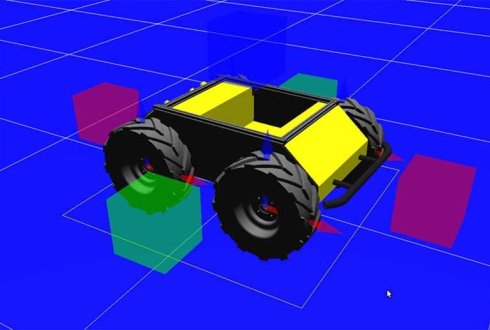
\includegraphics[height=0.5\textheight]{img/husky.jpg}
% \onslide<2>
% \centering
% \includegraphics[height=0.72\textheight]{tests/{res_ROS}.png}
% \onslide<3>
% \centering
% \includegraphics[height=0.72\textheight]{tests/{res_ROS_path}.pdf}
% \end{overprint}
% \end{center}
% \end{frame}

\begin{frame}{Results - Real Data - Parque O'Higgins}
\begin{center}
\small 
\vspace{-13pt}
\begin{tabular}{|c|c|c|c|c|c|c|c|c|c|c|c|}
\hline
$n_p$ & $n_l$ & $i_{op}$ & $i_{oa}$ & $i_{lp}$ & $it$ & $k_w$ & $\chi$ & $dt$ & $io$ & $ps$ & $t$\\
\hline \hline
8130 & 174 & 100000 & 100000 & 100 & 10 & 1 & $\infty$ & 3 & 500 & 10 & $4[hrs]$\\
\hline 
\end{tabular}
\begin{overprint}[\textwidth]
\onslide<1>
\centering
\vspace{4em}
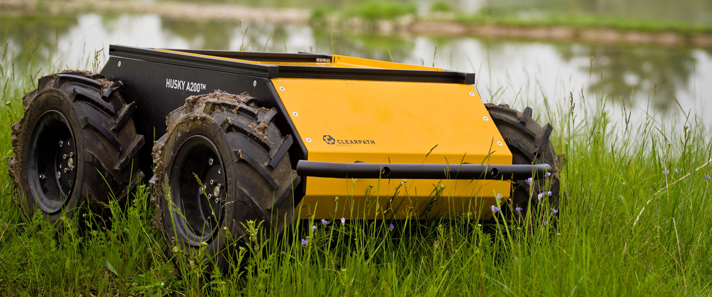
\includegraphics[height=0.4\textheight]{img/husky-grass.png}
\onslide<2>
\centering
\includegraphics[height=0.72\textheight]{tests/{res_ohiggins}.png}
\end{overprint}
\end{center}
\end{frame}

\begin{frame}{Results - Real Data - Victoria Park}
\begin{center}
\small 
\begin{tabular}{|c|c|c|c|c|c|c|c|c|c|c|c|}
\hline
$n_p$ & $n_l$ & $i_{op}$ & $i_{oa}$ & $i_{lp}$ & $it$ & $k_w$ & $\chi$ & $dt$ & $io$ & $ps$ & $t$\\
\hline \hline
61763 & - & 8000 & 100000 & 5 & 15 & 1 & $\infty$ & 5 & 500 & 10 & $10[hrs]$\\
\hline 
\end{tabular}
\begin{overprint}[\textwidth]
\onslide<1>
\centering
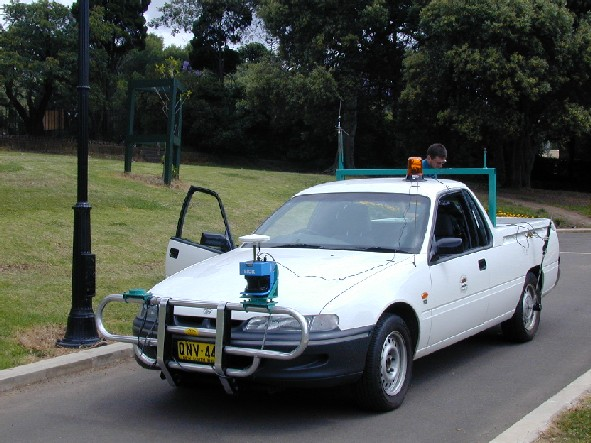
\includegraphics[height=0.72\textheight]{img/victoria.jpg}
\onslide<2>
\centering
\includegraphics[height=0.72\textheight]{tests/{res_victoria}.png}
\onslide<3>
\vspace{1em}
\centering
\begin{columns}
\column{0.5\textwidth}
\centering
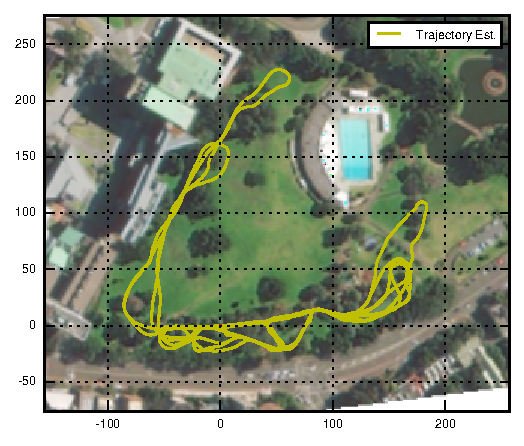
\includegraphics[width=0.9\textwidth]{img/estimate.pdf}\\
GraphSLAM
\column{0.5\textwidth}
\centering
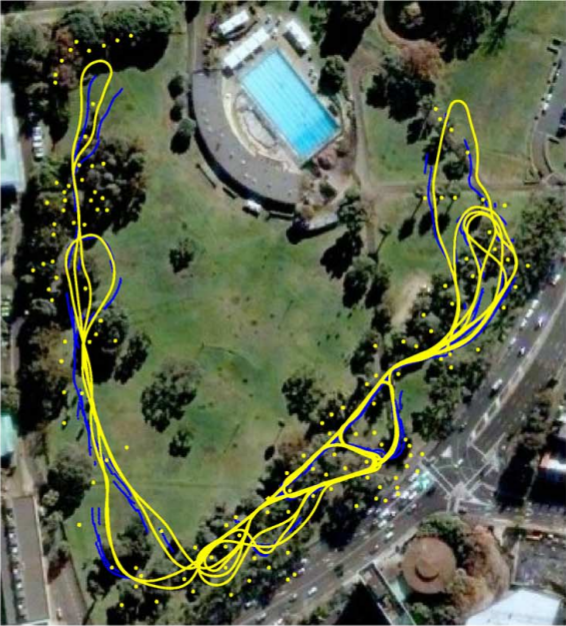
\includegraphics[width=0.63\textwidth, angle=-36]{img/victoria-isam.png}\\
iSAM
\end{columns}
\end{overprint}
\end{center}
\end{frame}

\begin{frame}{Conclusions}
\begin{itemize}
\setlength\itemsep{1.5em}
\item GraphSLAM was successfully implemented for the 2D scenario using \textbf{g$^2$o}.
\item A \textbf{correspondence test} was implemented to deal with the correspondence problem.
\item The \textbf{distant test} is used to speed up the algorithm.
\item The implementation works in the \textbf{known} and \textbf{unknown data association}, for \textbf{simulated} and \textbf{real data}.
\item The biggest drawbacks are the \textbf{computational time} and the \textbf{false positives}.
\item \textbf{Repository}: \url{https://github.com/francocurotto/GraphSLAM}.
\end{itemize}
\end{frame}

\begin{frame}{References}
\begin{thebibliography}{4}
\bibitem{} Thrun, Sebastian, and Michael Montemerlo. ``The graph SLAM algorithm with applications to large-scale mapping of urban structures.'' \textit{The International Journal of Robotics Research} 25.5-6 (2006): 403-429.
\bibitem{} Kümmerle, Rainer, et al. ``g 2 o: A general framework for graph optimization.'' \textit{Robotics and Automation (ICRA), 2011 IEEE International Conference on}. IEEE, 2011.
\bibitem{} Kaess, Michael, Ananth Ranganathan, and Frank Dellaert. ``iSAM: Incremental smoothing and mapping.'' \textit{Robotics, IEEE Transactions on} 24.6 (2008): 1365-1378.
\bibitem{} Thrun, Sebastian, Wolfram Burgard, and Dieter Fox. \textit{Probabilistic robotics}. MIT press, 2005.
\end{thebibliography}
\end{frame}

\begin{frame}
\author{
\vspace{-1em}
\hspace{-4em}
\begin{tabular}{rl} 
 \textbf{Author:}  & Franco Curotto \\
 \textbf{Thesis Adviser:} & Martin Adams \\ 
 \textbf{Commission Members:} & Marcos Orchard \\
 & Jorge Silva
\end{tabular}
\vspace{0em}
}
    
\includegraphics[width=0.4\textwidth]{img/fcfm_die.pdf}
    \titlepage
\end{frame}

\end{document}
